\documentclass[tikz,border=12pt]{standalone}
% Shared visual language for standalone EMT block diagrams.
\usepackage{amsmath}
\usetikzlibrary{arrows.meta,backgrounds,calc,fit,positioning}

\tikzset{
    emt diagram/.style = {>={Stealth[length=2.4mm]}},
    line/.style        = {semithick, rounded corners=6pt},
    block/.style       = {draw, semithick, fill=white,
                          minimum height=1cm, minimum width=2.3cm},
    hblock/.style      = {block, minimum width=2.24cm, minimum height=1.3cm},
    vblock/.style      = {block, minimum width=1.3cm, minimum height=2.24cm},
    sum/.style         = {draw, semithick, fill=white, circle,
                          inner sep=2.6pt},
    signal/.style      = {circle, fill, inner sep=1.4pt,
                          label distance=3pt},
    sig/.style         = {font=\small},
    pm/.style          = {font=\scriptsize},
    wire jump/.style   = {line,
                          preaction={draw=white, line width=3pt,
                                     line cap=round}},
    enclosure/.style   = {draw, dashed, semithick, rounded corners=4pt},
    operator enclosure/.style = {enclosure, inner xsep=7mm, inner ysep=6mm}
}


\begin{document}
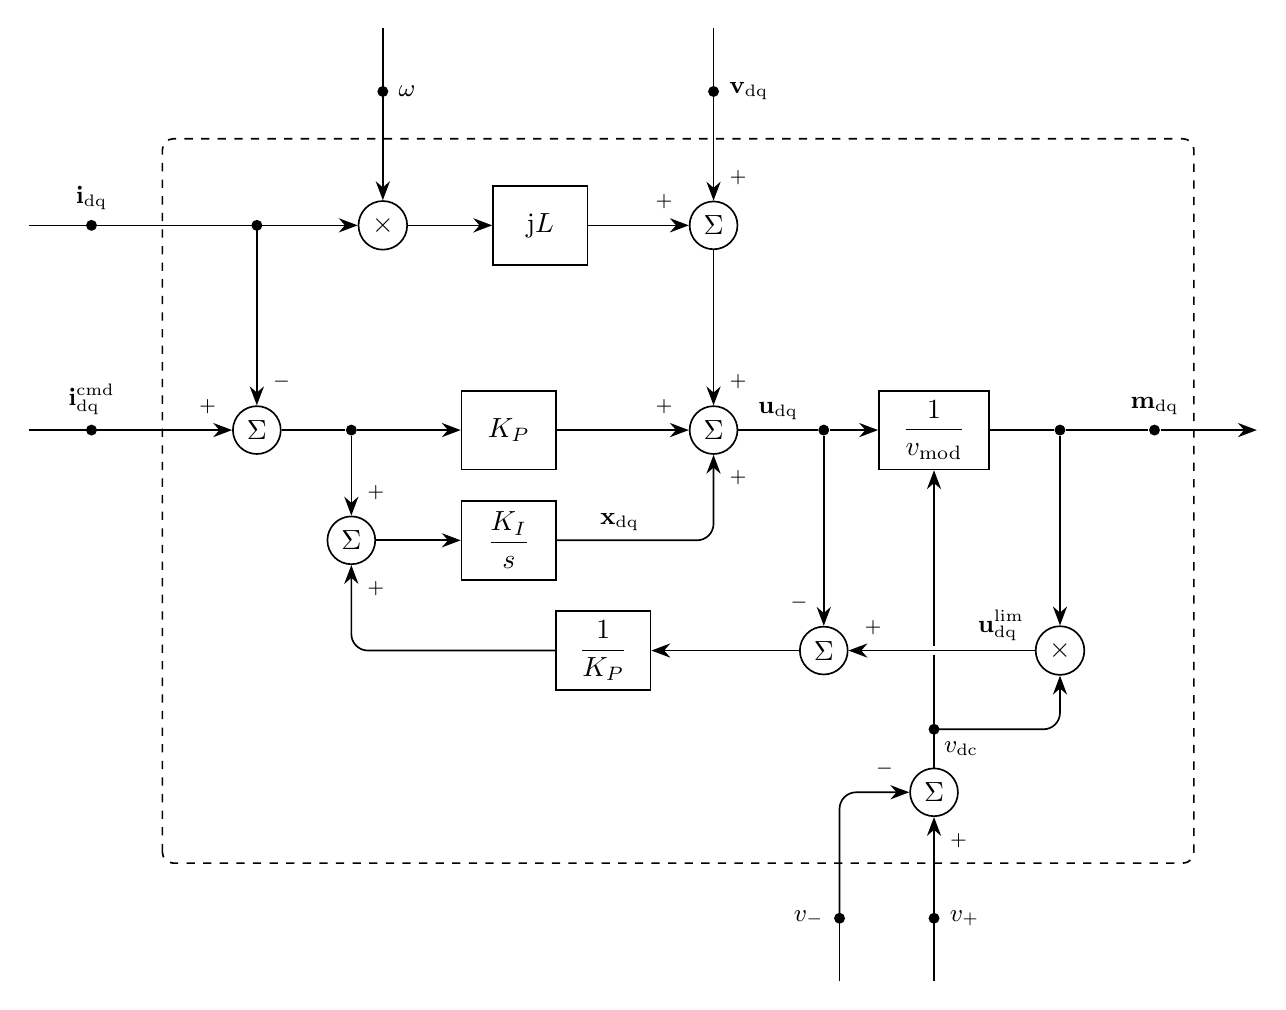
\begin{tikzpicture}[emt diagram]

\coordinate (iin) at (-0.9,3.6);
\coordinate (icmdin) at (-0.9,1.0);
\coordinate (omegain) at (2.8,5.3);
\coordinate (vin) at (7.0,5.3);
\coordinate (vposin) at (9.8,-5.2);
\coordinate (vnegin) at (8.6,-5.2);

% Current error, proportional path, and integrator.
\coordinate (isplit) at (1.2,3.6);
\node[sum] (err) at (1.2,1.0) {$\Sigma$};
\node[signal] (errsplit) at (2.4,1.0) {};
\node[block, minimum width=1.2cm] (kp) at (4.4,1.0) {$K_P$};
\node[sum] (aw) at (2.4,-0.4) {$\Sigma$};
\node[block, minimum width=1.2cm] (ki) at (4.4,-0.4) {$\dfrac{K_I}{s}$};

% Decoupling and voltage feedforward.
\node[sum] (speed) at (2.8,3.6) {$\times$};
\node[block, minimum width=1.2cm] (cross) at (4.8,3.6) {$\mathrm{j}L$};
\node[sum] (ff) at (7.0,3.6) {$\Sigma$};
\node[sum] (usum) at (7.0,1.0) {$\Sigma$};

% Voltage limit.
\node[signal] (usplit) at (8.4,1.0) {};
\node[block, minimum width=1.4cm] (limit) at (9.8,1.0) {$\dfrac{1}{v_\mathrm{mod}}$};
\node[signal] (msplit) at (11.4,1.0) {};

% Limited-voltage feedback to the integrator.
\node[sum] (excess) at (8.4,-1.8) {$\Sigma$};
\node[block, minimum width=1.2cm] (kpinv) at (5.6,-1.8) {$\dfrac{1}{K_P}$};
\node[sum] (dc) at (9.8,-3.6) {$\Sigma$};
\coordinate (vdcsplit) at (9.8,-2.8);

% Vertical wires first; horizontal wires jump over them.
\draw[->, line] (isplit) -- (err.north);
\draw[line] (dc.north) -- (vdcsplit)
    node[sig, midway, right] {$v_\mathrm{dc}$};
\draw[->, line] (vdcsplit) -- (limit.south);

\draw[line] ($(iin)+(-0.8,0)$) -- (iin);
\draw[->, line] (iin) -- (speed.west);
\draw[line] ($(icmdin)+(-0.8,0)$) -- (icmdin);
\draw[->, line] (icmdin) -- (err.west);
\draw[line] ($(omegain)+(0,0.8)$) -- (omegain);
\draw[->, line] (omegain) -- (speed.north);
\draw[line] ($(vin)+(0,0.8)$) -- (vin);
\draw[->, line] (vin) -- (ff.north);

\draw[->, line] (speed.east) -- (cross.west);
\draw[->, line] (cross.east) -- (ff.west);
\draw[->, line] (ff.south) -- (usum.north);

\draw[line] (err.east) -- (errsplit);
\draw[->, line] (errsplit) -- (kp.west);
\draw[->, line] (kp.east) -- (usum.west);
\draw[->, line] (errsplit) -- (aw.north);
\draw[->, line] (aw.east) -- (ki.west);
\draw[->, line] (ki.east) -- (7.0,-0.4)
    node[sig, pos=0.4, above] {$\mathbf{x}_\mathrm{dq}$} -- (usum.south);

\draw[line] (usum.east) -- (usplit)
    node[sig, midway, above] {$\mathbf{u}_\mathrm{dq}$};
\draw[->, line] (usplit) -- (limit.west);
\draw[line] (limit.east) -- (msplit);
\node[signal, label={[sig]above:$\mathbf{m}_\mathrm{dq}$}] (mout) at (12.6,1.0) {};
\draw[line] (msplit) -- (mout);
\draw[->, line] (mout) -- ++(1.3,0);

\draw[->, line] (usplit) -- (excess.north);
% The product node follows its output wire so the halo stays under it.
\draw[->, wire jump] (11.4,-1.8) -- (excess.east)
    node[sig, pos=0.28, above] {$\mathbf{u}_\mathrm{dq}^\mathrm{lim}$};
\node[sum] (product) at (11.4,-1.8) {$\times$};
\draw[->, line] (msplit) -- (product.north);
\draw[->, line] (excess.west) -- (kpinv.east);
\draw[->, line] (kpinv.west) -| (aw.south);
\draw[->, line] (vdcsplit) -| (product.south);

\draw[line] ($(vposin)+(0,-0.8)$) -- (vposin);
\draw[->, line] (vposin) -- (dc.south);
\draw[line] ($(vnegin)+(0,-0.8)$) -- (vnegin);
\draw[->, line] (vnegin) |- (dc.west);

% Signs at each summing junction.
\node[pm, anchor=south east] at ($(err.west)+(-0.08,0.08)$) {$+$};
\node[pm, anchor=south west] at ($(err.north)+(0.08,0.08)$) {$-$};
\node[pm, anchor=south west] at ($(aw.north)+(0.08,0.08)$) {$+$};
\node[pm, anchor=north west] at ($(aw.south)+(0.08,-0.08)$) {$+$};
\node[pm, anchor=south east] at ($(ff.west)+(-0.08,0.08)$) {$+$};
\node[pm, anchor=south west] at ($(ff.north)+(0.08,0.08)$) {$+$};
\node[pm, anchor=south east] at ($(usum.west)+(-0.08,0.08)$) {$+$};
\node[pm, anchor=south west] at ($(usum.north)+(0.08,0.08)$) {$+$};
\node[pm, anchor=north west] at ($(usum.south)+(0.08,-0.08)$) {$+$};
\node[pm, anchor=south east] at ($(excess.north)+(-0.08,0.08)$) {$-$};
\node[pm, anchor=south west] at ($(excess.east)+(0.08,0.08)$) {$+$};
\node[pm, anchor=north west] at ($(dc.south)+(0.08,-0.08)$) {$+$};
\node[pm, anchor=south east] at ($(dc.west)+(-0.08,0.08)$) {$-$};

% Junction and input dots last so wire halos never cover them.
\foreach \p in {(isplit),(vdcsplit)}
    \node[signal] at \p {};
\node[signal, label={[sig]above:$\mathbf{i}_\mathrm{dq}$}] at (iin) {};
\node[signal, label={[sig]above:$\mathbf{i}_\mathrm{dq}^\mathrm{cmd}$}] at (icmdin) {};
\node[signal, label={[sig]right:$\omega$}] at (omegain) {};
\node[signal, label={[sig]right:$\mathbf{v}_\mathrm{dq}$}] at (vin) {};
\node[signal, label={[sig]right:$v_+$}] at (vposin) {};
\node[signal, label={[sig]left:$v_-$}] at (vnegin) {};

\draw[enclosure] (0,-4.5) rectangle (13.1,4.7);

\end{tikzpicture}
\end{document}
